\documentclass{beamer}

\usepackage[utf8]{inputenc} 
\usepackage[T1]{fontenc}
\usepackage{lmodern}
\usepackage{graphicx}
\usepackage[french]{babel}
\usepackage{listings}

\usetheme{Warsaw}

% \definecolor{color1}{RGB}{33,33,33}
% \definecolor{color2}{RGB}{222,69,0}
\definecolor{color3}{RGB}{239,239,239}
% \definecolor{color4}{RGB}{0,119,170}
\setbeamercolor{background canvas}{bg=color3}



\begin{document}

\title{Présentation Bash Build}
\subtitle[\ldots]{Soutenance Projet}
\author[Aymerick LAURETTA-PERONNE]{Aymerick LAURETTA-PERONNE}
\institute[France]{France/Guadeloupe}
\date{\today}
\maketitle

\begin{frame} % 1er Diapo
\frametitle{Introduction}
\framesubtitle{Description}

Bash-Build est un jeu de construction codé en langage C et s’exécutant dans un terminal. Il dispose d’une interface ergonomique composée de multiples menus interactifs permettant de naviguer dans les fonctionnalités.

\end{frame}

\begin{frame} % 2e Diapo
\frametitle{Présentation}
\framesubtitle{Declaration Structure}
    \begin{center}
        % 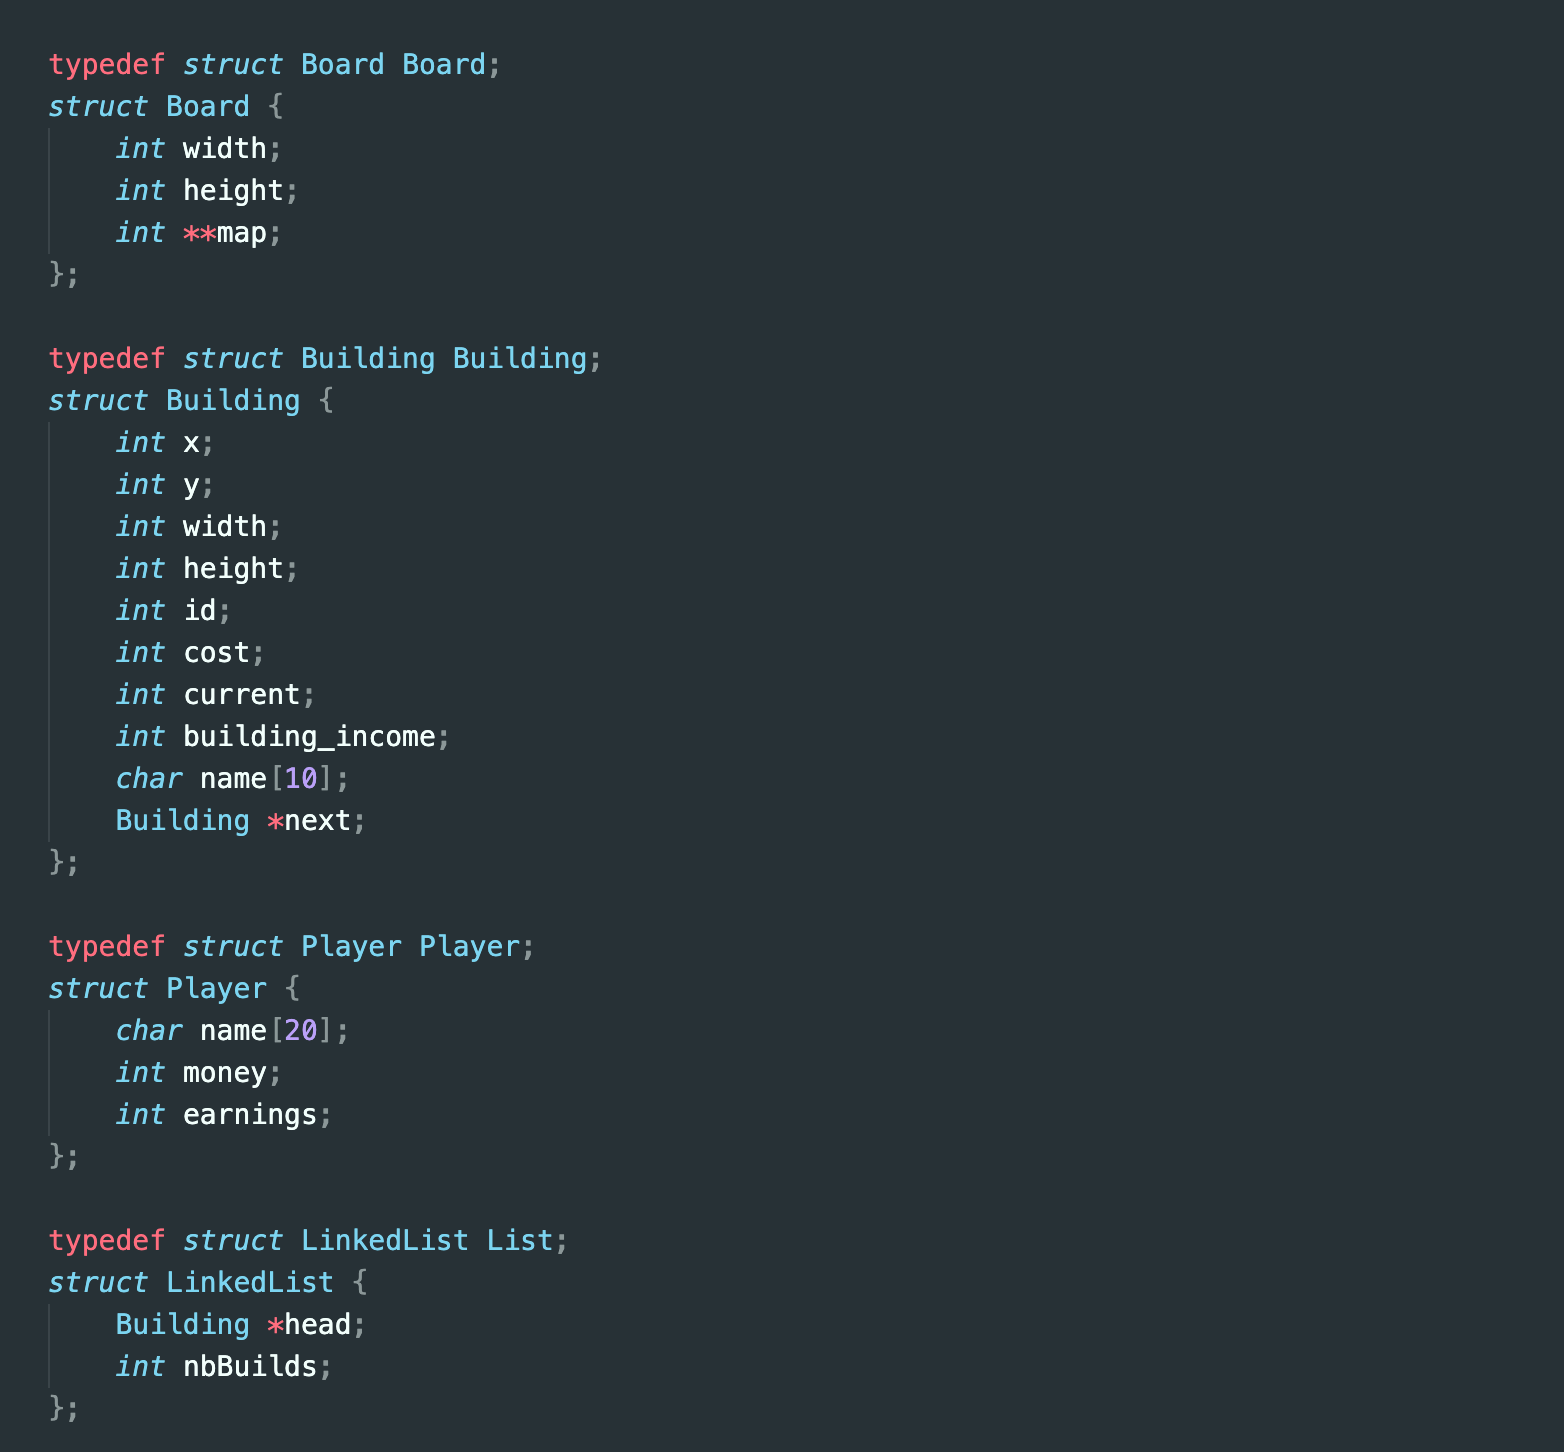
\includegraphics[scale=0.28]{src/images/struct.png}
        \begin{lis}
    \end{center}
\end{frame}

\begin{frame} % 3e Diapo
\frametitle{Présentation}
\framesubtitle{Declaration Fonction en tant que prototype}

\begin{center}
    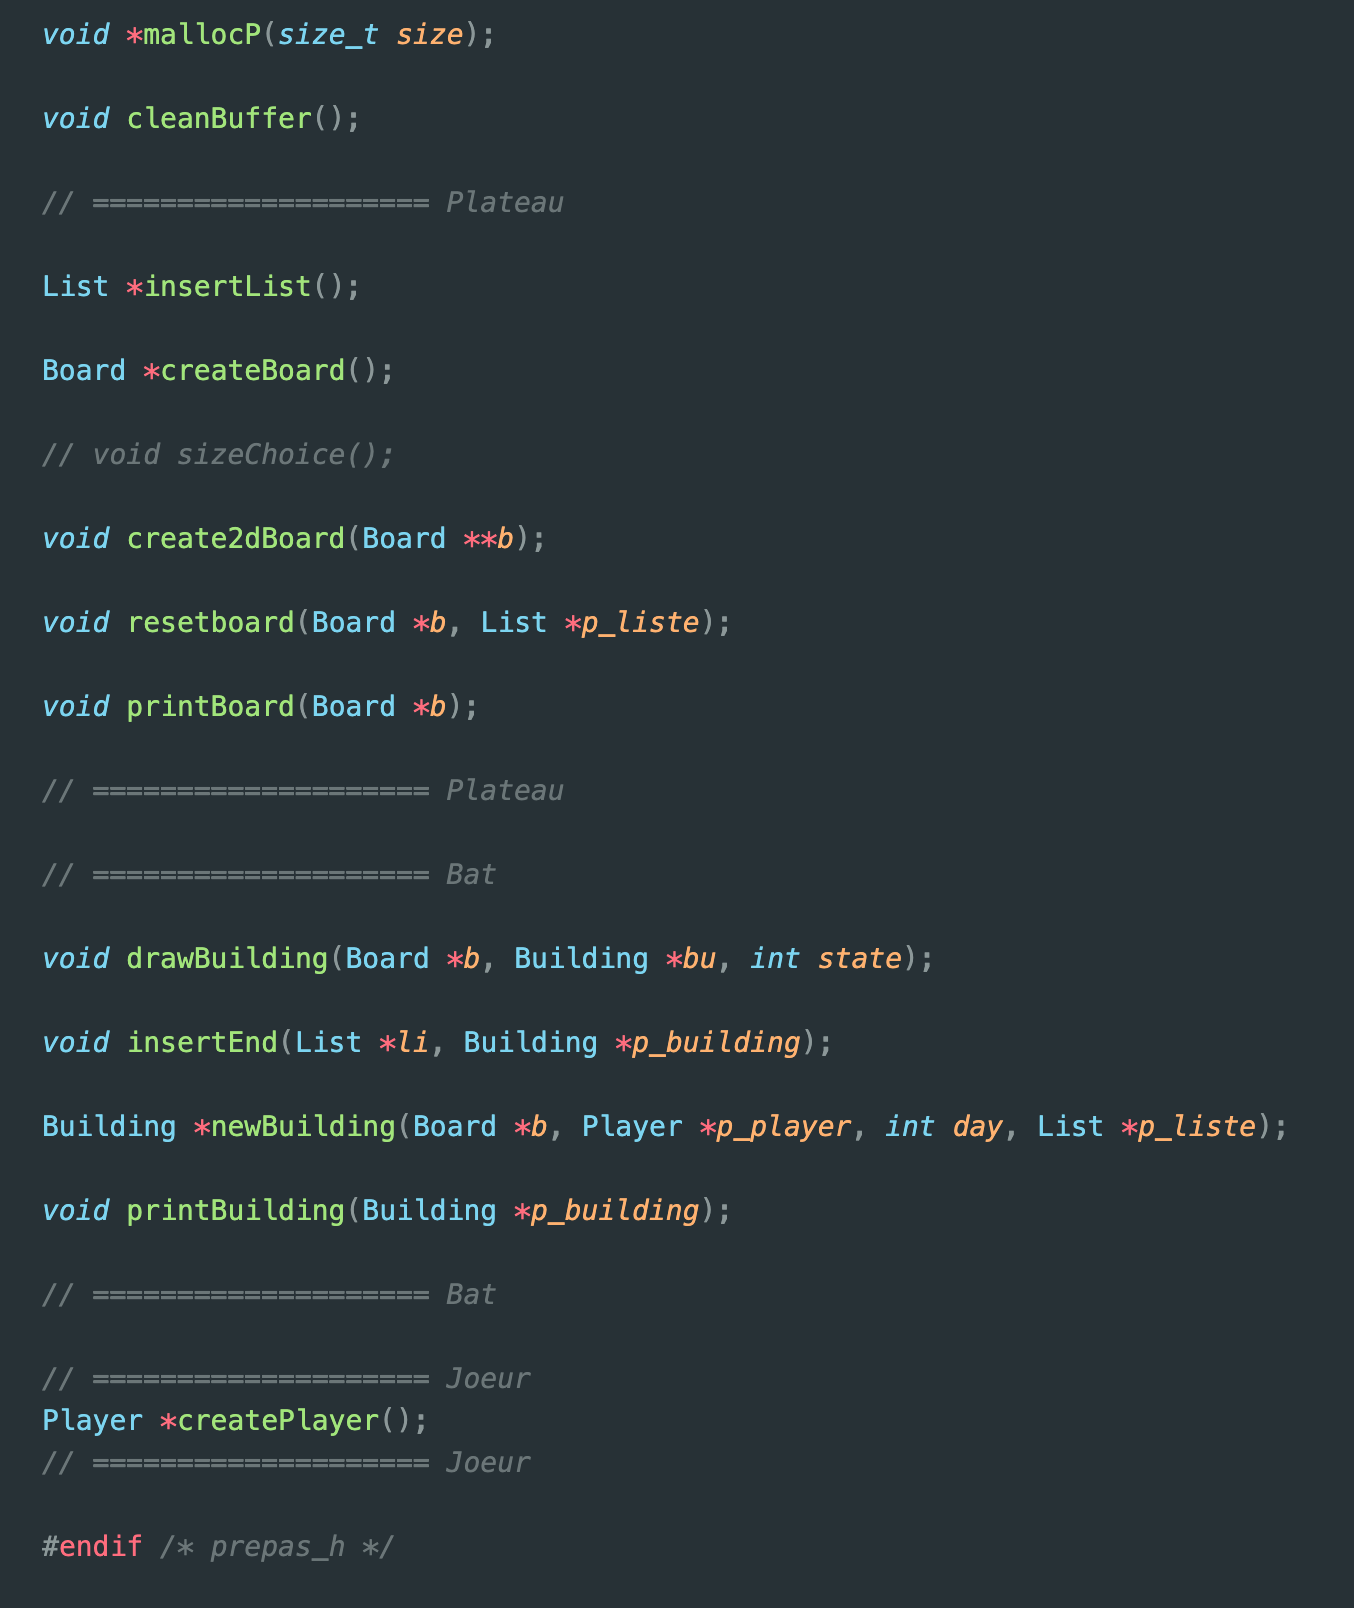
\includegraphics[scale=0.25]{src/images/declaration_fonction_as_prototype.png}
\end{center}

\end{frame}

\begin{frame} % 4e Diapo
    \frametitle{Présentation}
    \framesubtitle{Menu}
    
    \begin{center}
        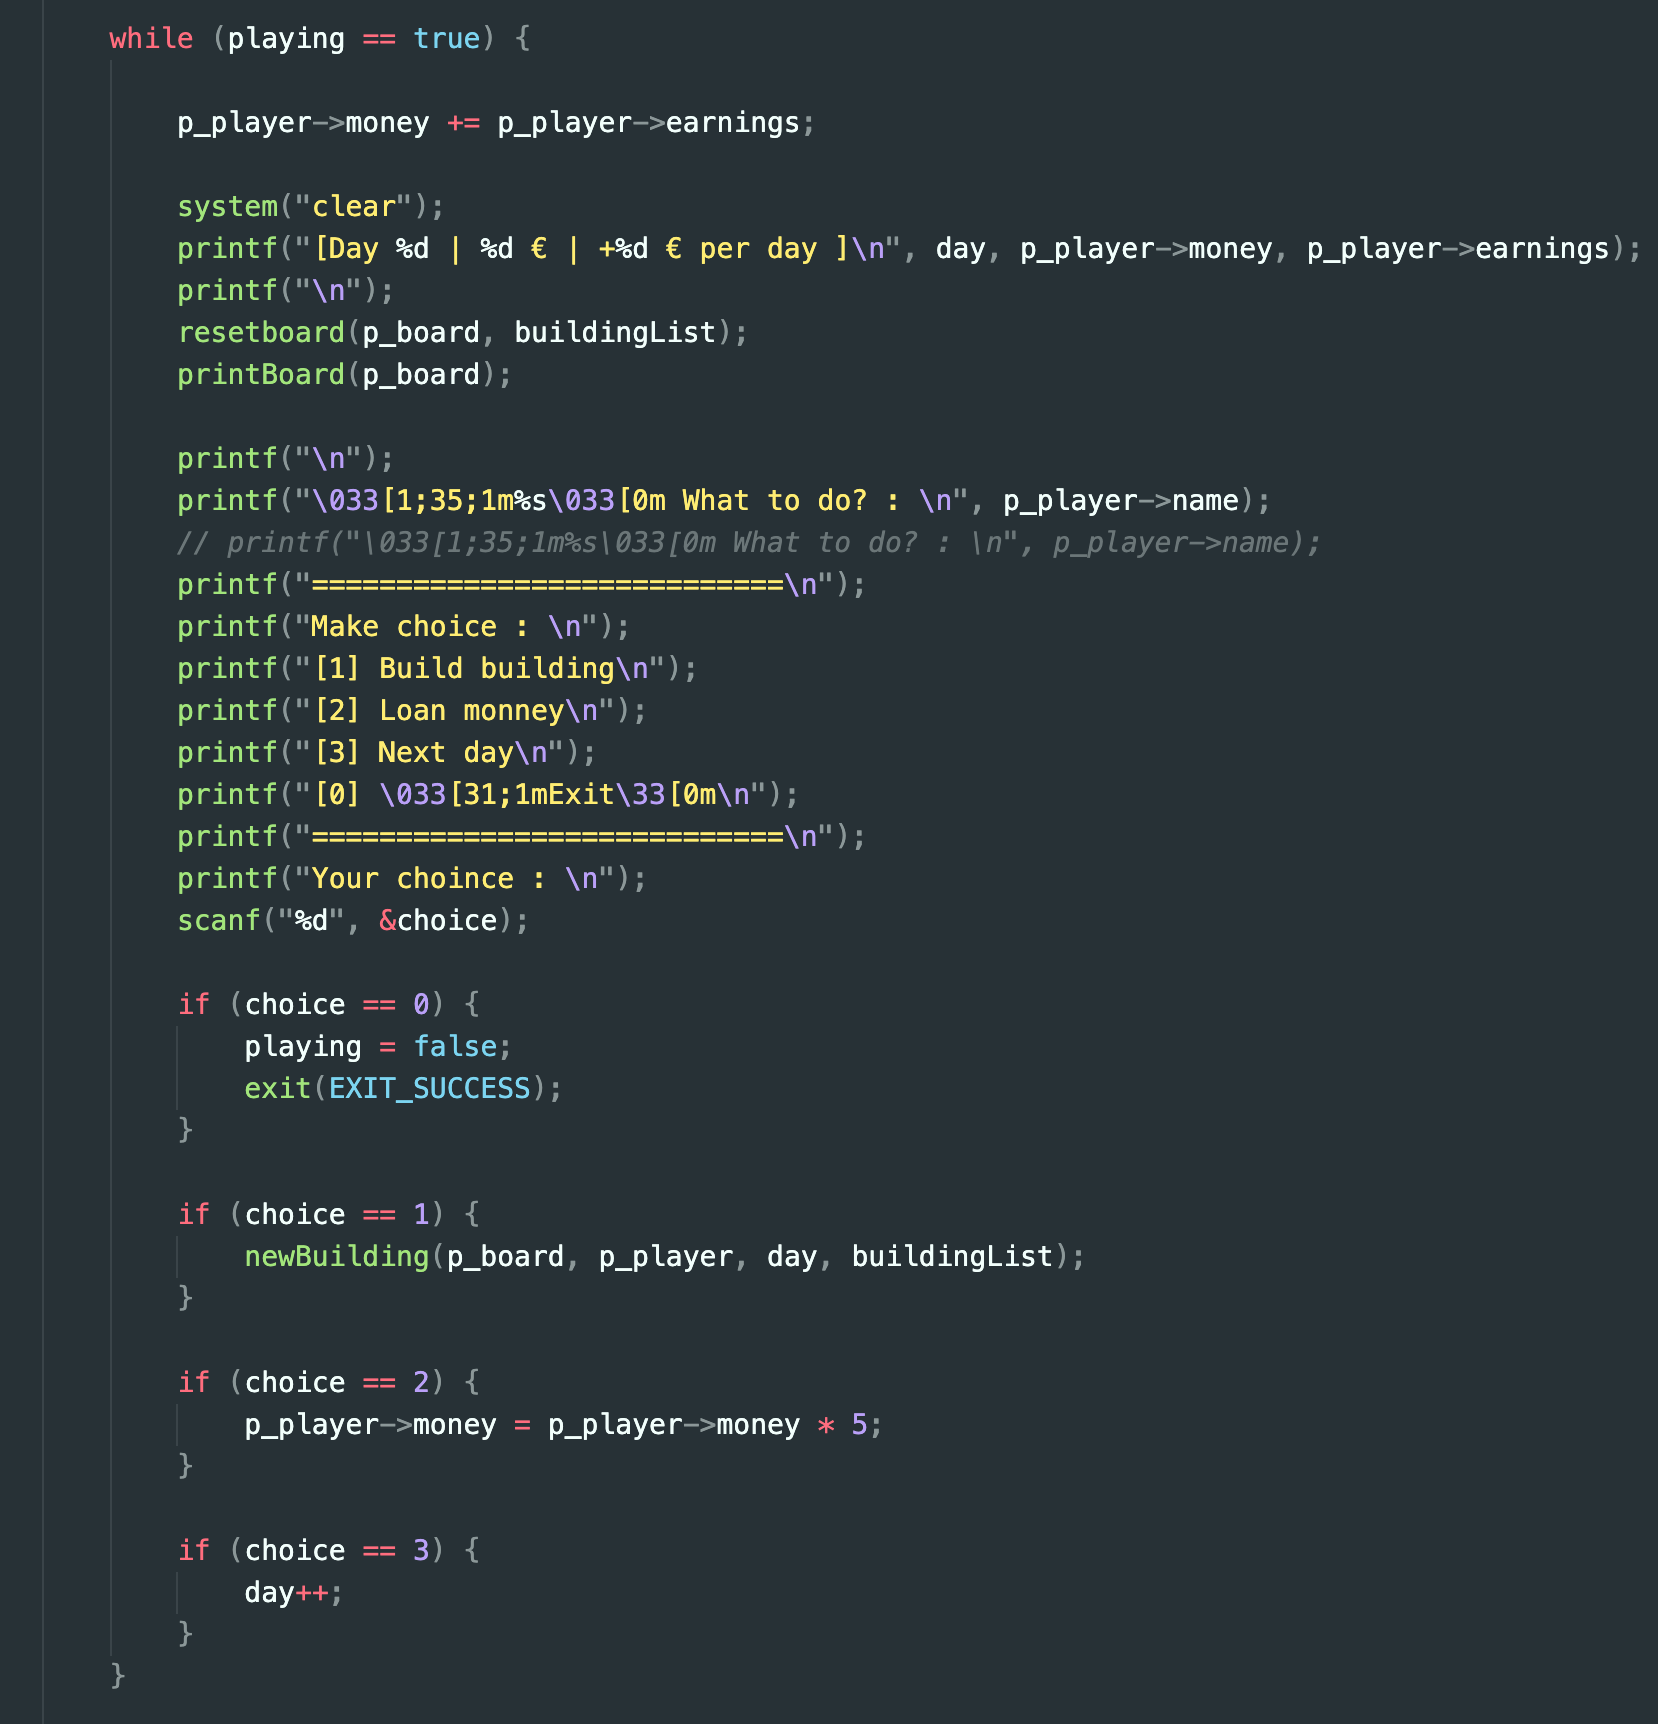
\includegraphics[scale=0.24]{src/images/menu.png}
    \end{center}
    
    \end{frame}

\end{document}
